\documentclass[tikz]{standalone}


\begin{document}
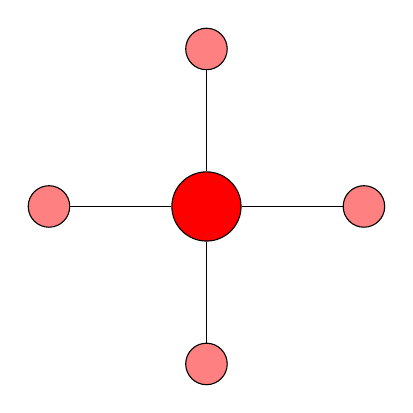
\begin{tikzpicture}[scale=2]
  \tikzset{ nbh/.style={draw, circle, fill=red!50, minimum width=15pt} };
  \node[circle,draw,fill=red, minimum width=25pt] (A) {};
  \draw (A) -- ++(-1,+0) node[nbh] {};
  \draw (A) -- ++(+0,-1) node[nbh] {};
  \draw (A) -- ++(+0,+1) node[nbh] {};
  \draw (A) -- ++(+1,+0) node[nbh] {};
\end{tikzpicture}
\end{document}
